\documentclass[11pt,a4paper]{article}

\usepackage[spanish,es-noshorthands,es-tabla]{babel}
\usepackage{lmodern}
\usepackage[margin=2.4cm]{geometry}
\usepackage{graphicx}
\usepackage{booktabs}
\usepackage{tabularx}
\usepackage{array}
\usepackage{amsmath}
\usepackage{xcolor}
\usepackage{enumitem}
\usepackage{caption}
\usepackage{float}
\usepackage{tikz}
\usetikzlibrary{positioning,arrows.meta}
\usepackage{xurl}
\usepackage[hidelinks]{hyperref}

\definecolor{azul}{HTML}{2A78D6}
\definecolor{tinta}{HTML}{52514E}
\definecolor{fondo}{HTML}{F3F2EF}

\setlist{itemsep=2pt,topsep=4pt}
\captionsetup{font=small,labelfont=bf}
\newcolumntype{L}{>{\raggedright\arraybackslash}X}

\newcommand{\aviso}[1]{%
  \begin{center}\fcolorbox{tinta}{fondo}{\parbox{0.92\linewidth}{\small #1}}\end{center}}

\title{\textbf{Estimación de riesgo de grooming\\a partir de la edad aparente de la voz}\\[4pt]
\large Reporte técnico del proyecto (versión 2)}
\author{}
\date{Octubre de 2026}

\begin{document}
\maketitle

%=====================================================================
\begin{abstract}
%=====================================================================
\noindent\textbf{Resumen.}
El grooming en línea ---el proceso por el que una persona adulta se gana la confianza de una persona menor de edad con fines sexuales--- crece año con año y se desplaza a espacios con voz, como los videojuegos en línea y las llamadas. Este trabajo presenta un sistema que, usando \emph{solo la voz}, estima si en una conversación participan una persona menor de edad y una adulta, sin transcribir ni analizar lo que se dice. El sistema separa a los hablantes, estima para cada uno la probabilidad de ser niño (12 años o menos), adolescente (13--17) o adulto (18 o más) y combina esas probabilidades en un puntaje de riesgo. Se compararon seis modelos de aprendizaje de máquina ---tres representaciones de la voz (rasgos acústicos clásicos, vectores de hablante ECAPA-TDNN y la red autosupervisada WavLM) con distintos clasificadores--- sobre 23\,893 fragmentos de audio (27,7 horas) de dos corpus públicos en inglés, con partición estricta por hablante. El mejor modelo, ECAPA-TDNN con una máquina de vectores de soporte, alcanza un F1-macro de 0,817 por fragmento, detecta el 98,7\,\% de los fragmentos infantiles y el 60,4\,\% de los adolescentes, y separa menores de adultos con un AUC de 0,943. En conversaciones simuladas niño--adulto genera alerta alta en el 80\,\% de los casos, sin alertas altas en los escenarios sin pareja menor--adulto. El resultado es una \textbf{alerta para priorizar revisión humana}, nunca una prueba de que exista grooming.
\end{abstract}

\aviso{\textbf{Principio rector: es una alerta, no un decisor.} Que un menor hable con un adulto no es grooming: padres, docentes, médicos y entrenadores producen exactamente la misma señal. Un riesgo de 90\,\% significa ``el modelo está bastante seguro de que hay un niño y un adulto distintos'', no ``90\,\% de probabilidad de grooming''. Ninguna acción con consecuencias debe tomarse solo con este puntaje.}

\tableofcontents
\newpage

%=====================================================================
\section{Introducción}
%=====================================================================

El \emph{grooming} en línea es el proceso mediante el cual una persona adulta establece contacto y confianza con una persona menor de edad, a través de medios digitales, para facilitar un abuso sexual~\cite{whittle2013}. Suele avanzar por etapas ---contacto, construcción de confianza, aislamiento, sexualización--- y aprovecha plataformas donde los menores pasan tiempo: redes sociales, mensajería y videojuegos en línea.

\subsection{La magnitud del problema}

\begin{table}[H]
\centering
\caption{Indicadores recientes sobre explotación y grooming en línea.}
\label{tab:estadisticas}
\small
\begin{tabularx}{\linewidth}{@{}>{\raggedright\arraybackslash}p{3.0cm}Lp{1.7cm}@{}}
\toprule
\textbf{Fuente} & \textbf{Dato} & \textbf{Periodo} \\
\midrule
NCMEC / Thorn (EE.\,UU.) & Los reportes de \emph{incitación en línea} (un adulto que se comunica con un menor con fines sexuales) subieron 192\,\%, a más de 546\,000~\cite{thorn2025}; en 2023 habían sido unos 186\,800~\cite{ncmec2025}. & 2024 \\
NCMEC & Casi 100 reportes \emph{al día} de extorsión sexual con fines económicos; al menos 36 adolescentes varones se han quitado la vida tras ser víctimas desde 2021~\cite{ncmec2025}. & 2024 \\
NSPCC (Reino Unido) & 7\,263 delitos de comunicación sexual con un menor registrados por la policía, casi el doble que en 2017/18; el 40\,\% de los casos con plataforma identificada ocurrió en Snapchat~\cite{nspcc2025}. & 2024/25 \\
WeProtect Global Alliance & En plataformas de videojuegos, una conversación puede volverse grooming de alto riesgo en 45 minutos en promedio, y en tan solo 19 segundos~\cite{weprotect2023}. & 2023 \\
WeProtect Global Alliance & Aumento de 87\,\% en reportes de material de abuso sexual infantil desde 2019~\cite{weprotect2023}. & 2019--2023 \\
INEGI, MOCIBA (México) & 21,0\,\% de las personas usuarias de internet de 12 años o más ---18,9 millones--- vivió ciberacoso; la forma más común fue el contacto mediante identidades falsas, y los medios principales, WhatsApp (39,8\,\%) y Facebook (39,7\,\%)~\cite{inegi2025}. & 2024 \\
\bottomrule
\end{tabularx}
\end{table}

Dos matices al leer estas cifras. Parte del salto de 2024 en Estados Unidos se debe a la \emph{REPORT Act}, que volvió obligatorio reportar la incitación en línea~\cite{thorn2025}: refleja más casos visibles, no necesariamente más casos. Y la cifra de México mide ciberacoso en general, del cual el grooming es una forma particular.

\subsection{Por qué la voz}

La mayoría de las herramientas de detección automática analizan texto de chats (sección~\ref{sec:trabajos}). Pero el contacto ocurre cada vez más por voz: chats de voz en videojuegos, notas de voz y llamadas. La voz tiene además una propiedad útil: \textbf{delata la edad aproximada del hablante}, porque los niños tienen cuerdas vocales y tracto vocal más cortos, lo que eleva el tono y las resonancias de la voz (sección~\ref{sec:marco}). Este proyecto aprovecha esa señal para detectar la \emph{condición previa} del grooming ---que un menor y un adulto estén hablando---, sin necesidad de escuchar qué dicen.

\subsection{Por qué el sistema no analiza lo que se dice}

Una decisión central del diseño es que el sistema \textbf{no transcribe ni interpreta el contenido} de la conversación; solo mide rasgos acústicos de la voz relacionados con la edad. Las razones:

\begin{enumerate}
  \item \textbf{Privacidad y confidencialidad de las comunicaciones.} Analizar el contenido de conversaciones privadas es una de las intervenciones más intrusivas posibles. Las autoridades europeas de protección de datos (EDPB y EDPS) recomendaron eliminar la detección de grooming de la propuesta de reglamento europeo contra el abuso sexual infantil, por su carácter intrusivo, probabilístico y sus tasas de error, y fueron especialmente críticas con el escaneo de comunicaciones de \emph{audio}, que exigiría interceptación continua y en vivo~\cite{edpb2022}. Nuestro enfoque evita ese escaneo de contenido por diseño.
  \item \textbf{Minimización de datos.} De cada hablante solo se conservan tres probabilidades (niño, adolescente, adulto). No se generan transcripciones, no se guardan audios ni se identifica a nadie.
  \item \textbf{Proporcionalidad.} Una alerta basada en la edad aparente permite priorizar casos sin exponer lo que dijeron menores y adultos inocentes, que serán la mayoría de las alertas.
  \item \textbf{Independencia del idioma.} Las pistas de edad (tono y formantes) dependen de la fisiología, no del idioma ni del vocabulario.
  \item \textbf{Menor superficie de riesgo.} Un sistema que nunca produce texto de las conversaciones no puede filtrarlo, ni usarse para vigilar lo que la gente dice.
\end{enumerate}

\textbf{El costo de esta decisión}, que debe decirse con claridad: el sistema no distingue una conversación legítima de una abusiva. Detecta la combinación ``menor + adulto'', no la intención. Por eso su salida es una alerta para revisión humana y nunca un veredicto.

\subsection{Objetivo y alcance}

\textbf{Objetivo.} Dado un audio de una conversación, estimar la probabilidad de que en él participen una persona menor de edad y una persona adulta distintas, para priorizar qué conversaciones debe revisar una persona especializada.

\textbf{Clases de edad:} \textbf{niño} (12 años o menos), \textbf{adolescente} (13 a 17 años) y \textbf{adulto} (18 años o más).

\textbf{Fuera del alcance.} El sistema no analiza el contenido de la conversación, no identifica a las personas y no decide si hay un delito. Tampoco toma acciones automáticas (bloqueos, denuncias).

\textbf{Contribuciones.} (1) Un flujo de punta a punta ---diarización, estimación de edad por hablante y puntaje de riesgo--- que funciona solo con CPU y sin conexión; (2) una comparación controlada de seis modelos con el mismo protocolo y partición por hablante; (3) una auditoría del sesgo por canal de grabación, y (4) un servicio web listo para desplegarse que no conserva audio.

%=====================================================================
\section{Trabajos relacionados}
\label{sec:trabajos}
%=====================================================================

\subsection{Detección automática de grooming}

La línea de investigación más establecida trabaja sobre \textbf{texto}. La competencia PAN 2012 de identificación de depredadores sexuales~\cite{pan2012} definió un corpus de conversaciones de chat y dos tareas: identificar a los depredadores y señalar sus mensajes problemáticos. El sistema ganador usó un enfoque en dos pasos ---primero filtrar las conversaciones sospechosas y después clasificar a los participantes--- con representaciones de bolsa de palabras~\cite{villatoro2012}. Trabajos posteriores aplicaron redes neuronales convolucionales a las mismas conversaciones~\cite{ebrahimi2016}. Todos estos enfoques requieren acceso al contenido de los mensajes y dependen del idioma; ninguno aborda la voz.

\subsection{Estimación de edad a partir de la voz}

La estimación automática de la edad del hablante es una tarea clásica de la paralingüística. Metze et~al.~\cite{metze2007} compararon cuatro enfoques para reconocer edad y género en aplicaciones telefónicas, con clases que incluían a niños. El \emph{INTERSPEECH 2010 Paralinguistic Challenge}~\cite{schuller2010} estandarizó la tarea con cuatro grupos de edad (niños, jóvenes, adultos y mayores) y un conjunto común de rasgos acústicos, y mostró que las clases intermedias son las más difíciles de separar. Con la llegada de los vectores de hablante, Bahari et~al.~\cite{bahari2014} estimaron la edad sobre \emph{i-vectors} y Ghahremani et~al.~\cite{ghahremani2018} propusieron redes neuronales de extremo a extremo basadas en \emph{x-vectors}~\cite{xvector2018}. Más recientemente, Burkhardt et~al.~\cite{burkhardt2023} ajustaron modelos Transformer autosupervisados (wav2vec\,2.0) para predecir edad y género, con resultados del estado del arte; ese modelo se usó en este proyecto solo como referencia, porque su licencia no permite uso comercial.

\subsection{Diarización de hablantes}

Para estimar la edad de cada participante primero hay que saber \emph{quién habla y cuándo}. Los sistemas modernos de diarización combinan detección de actividad de voz, vectores de hablante y agrupamiento, o bien redes neuronales de extremo a extremo~\cite{park2022}. Herramientas como pyannote.audio~\cite{pyannote2020} ofrecen modelos neuronales de alta calidad, pero requieren descargar modelos con registro y tienen un costo de cómputo mayor. Este proyecto usa una diarización ligera, basada en el mismo extractor ECAPA-TDNN del clasificador, para mantener el sistema autónomo.

\subsection{Diferencia con este trabajo}

Hasta donde sabemos, no hay trabajos públicos que combinen estimación de edad por voz y diarización para \emph{estimar el riesgo} de una pareja menor--adulto en una conversación. Este trabajo se ubica entre las dos líneas anteriores: toma de la paralingüística la estimación de edad y la aplica al problema del grooming, pero renuncia por diseño a analizar el contenido.

%=====================================================================
\section{Marco teórico}
\label{sec:marco}
%=====================================================================

\subsection{Producción de la voz y edad}

Según el modelo fuente--filtro~\cite{fant1960}, la voz resulta de una \textbf{fuente} ---la vibración de las cuerdas vocales--- cuyo sonido es moldeado por un \textbf{filtro}: el tracto vocal, que va de la laringe a los labios. Dos parámetros acústicos se derivan de esta descripción:

\begin{itemize}
  \item \textbf{Frecuencia fundamental ($F_0$)}, que percibimos como el tono. Depende de la longitud y masa de las cuerdas vocales: cuanto más cortas, más alta. En niños pequeños suele estar entre 250 y 300\,Hz o más; en adultos, alrededor de 120\,Hz en hombres y 210\,Hz en mujeres.
  \item \textbf{Formantes ($F_1$, $F_2$, $F_3$)}, las resonancias del tracto vocal. Si el tracto se modela como un tubo de longitud $L$ cerrado en un extremo, sus resonancias son
  \begin{equation}
    F_n = \frac{(2n-1)\,c}{4L}, \qquad n = 1, 2, 3, \dots
  \end{equation}
  donde $c \approx 350$\,m/s es la velocidad del sonido. Un tracto más corto ---como el de un niño--- produce formantes más altos.
\end{itemize}

Lee, Potamianos y Narayanan~\cite{lee1999} midieron estos parámetros en hablantes de 5 a 18 años: $F_0$ y formantes descienden con la edad, la variabilidad es mayor en los niños más pequeños y la mayoría de los valores converge al rango adulto hacia los 15 años, con la muda de la voz en los varones. Esto anticipa el reto central del problema: \textbf{distinguir niños de adultos es relativamente fácil, pero adolescentes y adultos se superponen}.

\subsection{Representaciones de la señal de voz}

\textbf{Rasgos acústicos clásicos.} Los \emph{coeficientes cepstrales en escala mel} (MFCC)~\cite{davis1980} resumen la envolvente espectral ---es decir, el filtro--- aplicando un banco de filtros con la resolución en frecuencia del oído humano, un logaritmo y una transformada coseno discreta. Junto con $F_0$, los formantes y otros rasgos espectrales forman un vector interpretable y barato de calcular.

\textbf{Vectores de hablante.} Una red neuronal entrenada para \emph{reconocer quién habla} aprende a resumir un audio de duración variable en un vector de longitud fija que captura timbre, tono y tamaño del tracto vocal. Los \emph{x-vectors}~\cite{xvector2018} introdujeron esta idea con redes de retardo temporal (TDNN). ECAPA-TDNN~\cite{ecapa2020} la mejora con tres elementos: bloques \emph{Res2Net} que analizan varias escalas temporales, bloques de compresión y excitación (\emph{squeeze-and-excitation}) que reponderan los canales, y un \emph{pooling} estadístico con atención que da más peso a los cuadros más informativos. Como la edad cambia esas mismas propiedades físicas, estos vectores son buenos candidatos para estimarla.

\textbf{Modelos autosupervisados.} WavLM~\cite{wavlm2022} es un Transformer preentrenado sin etiquetas con 94\,000 horas de habla: se enmascaran partes del audio, a veces mezclado con otra voz o ruido, y la red aprende a predecir las unidades ocultas. Cada capa codifica información distinta: las inferiores, rasgos acústicos y de hablante; las superiores, contenido lingüístico. Por eso en este trabajo se promedian las capas intermedias. WavLM lidera el banco de pruebas SUPERB en tareas de hablante y paralingüística~\cite{superb2021}.

\subsection{Clasificadores}

\begin{itemize}
  \item \textbf{Regresión logística:} modelo lineal que estima probabilidades con la función softmax. Sirve como referencia: si basta una frontera lineal, no hace falta más.
  \item \textbf{Máquina de vectores de soporte (SVM)}~\cite{svm1995}: busca la frontera que deja el \emph{margen máximo} entre clases. Con un núcleo de base radial (RBF), $k(\mathbf{x},\mathbf{x}') = \exp(-\gamma\lVert\mathbf{x}-\mathbf{x}'\rVert^2)$, la frontera puede ser no lineal. El parámetro $C$ controla cuánto se penalizan los errores de entrenamiento.
  \item \textbf{Bosque aleatorio}~\cite{rf2001}: promedia muchos árboles de decisión entrenados con muestras y rasgos al azar, lo que reduce la varianza.
  \item \textbf{Potenciación del gradiente}~\cite{friedman2001}: entrena árboles en secuencia, cada uno para corregir los errores de los anteriores.
\end{itemize}

\subsection{Calibración de probabilidades}

Un clasificador puede ordenar bien los casos y aun así dar probabilidades poco fiables. La \textbf{calibración sigmoide} o de Platt~\cite{platt1999} ajusta una función logística sobre las salidas del modelo en un conjunto de validación, de modo que una probabilidad de 0,9 acierte cerca del 90\,\% de las veces. Es indispensable aquí, porque el puntaje de riesgo multiplica probabilidades.

\subsection{Métricas de evaluación}

\begin{itemize}
  \item \textbf{Sensibilidad (\emph{recall}) por clase:} proporción de los ejemplos de una clase que el modelo reconoce. La de niños es la más importante, porque en una alerta el error más grave es no detectar al menor.
  \item \textbf{F1-macro:} promedio, sin ponderar, del F1 de cada clase (media armónica de precisión y sensibilidad). Trata por igual a todas las clases, aunque una tenga menos ejemplos.
  \item \textbf{Exactitud balanceada:} promedio de las sensibilidades de las tres clases.
  \item \textbf{AUC:} área bajo la curva ROC para separar menores (niños y adolescentes) de adultos; mide qué tan bien ordena el modelo, sin depender de un umbral.
\end{itemize}

%=====================================================================
\section{Metodología}
%=====================================================================

\subsection{Datos}

No existe un corpus público grande que tenga, en un mismo canal de grabación, voces de niños, adolescentes y adultos con edad etiquetada. Se unieron dos corpus públicos en inglés:

\begin{table}[H]
\centering
\caption{Corpus utilizados.}
\small
\begin{tabularx}{\linewidth}{@{}>{\raggedright\arraybackslash}p{3.6cm}L>{\raggedright\arraybackslash}p{2.0cm}p{1.9cm}@{}}
\toprule
\textbf{Corpus} & \textbf{Contenido} & \textbf{Edad} & \textbf{Clase} \\
\midrule
ENNI (habla infantil sintetizada)~\cite{enni2005,enniHF} & 9\,997 fragmentos de 349 niños de 4 a 10 años, generados a partir de narraciones reales; incluye niños con desarrollo típico y con trastorno del lenguaje & Exacta & Niño \\
Common Voice, década \emph{teens}~\cite{commonvoice2020} & Voluntarios grabados con micrófonos caseros & ``Menor de 19'' & Adolescente \\
Common Voice, década \emph{twenties} y mayores & 143\,170 fragmentos con edad declarada en total & Por década & Adulto \\
\bottomrule
\end{tabularx}
\end{table}

Las figuras~\ref{fig:enni} y~\ref{fig:cv} describen los corpus de origen. ENNI cubre de forma pareja los 4 a 10 años y ambos géneros, con unos 30 fragmentos por niño de 2 a 5\,s. Common Voice está muy desbalanceado: predominan los hombres de veinte a cuarenta años y los acentos de EE.\,UU. e Inglaterra, y la década \emph{teens} es de las más pequeñas.

\begin{figure}[H]
\centering
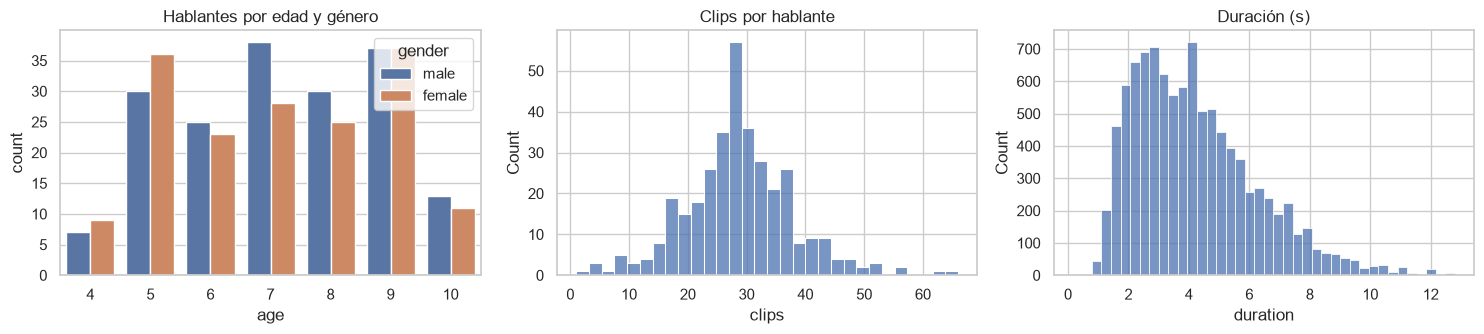
\includegraphics[width=\linewidth]{figuras/enni_hablantes_clips_duracion.png}
\caption{Corpus ENNI: hablantes por edad y género, fragmentos por hablante y duración de los fragmentos.}
\label{fig:enni}
\end{figure}

\begin{figure}[H]
\centering
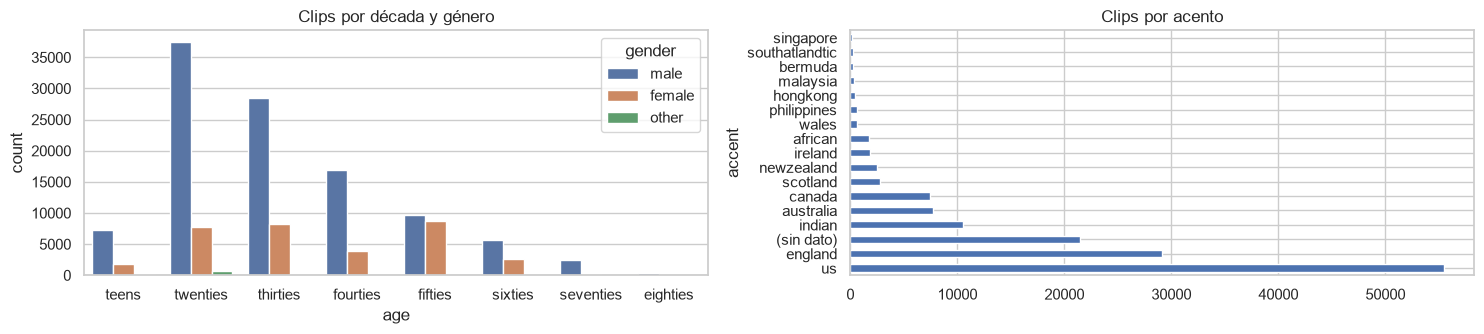
\includegraphics[width=\linewidth]{figuras/cv_clips_decada_acento.png}
\caption{Common Voice (fragmentos válidos con edad declarada): distribución por década y género, y por acento.}
\label{fig:cv}
\end{figure}

\textbf{Construcción del conjunto unido.}
\begin{enumerate}
  \item Se descartaron los fragmentos marcados como inválidos en Common Voice, los de menos de 1\,s o más de 15\,s y los fragmentos mudos.
  \item Como esta versión de Common Voice no identifica a los hablantes, se agruparon sus fragmentos en \emph{pseudo-hablantes} por década, género y acento. Una persona siempre declara los mismos datos, así que nunca queda repartida entre entrenamiento y prueba.
  \item Se limitaron los fragmentos por pseudo-hablante y se submuestreó a los adultos para equilibrar las clases.
  \item Todo se convirtió a audio mono de 16\,kHz.
\end{enumerate}

El resultado: \textbf{23\,893 fragmentos y 27,7 horas}: 9\,970 de niños (11,6\,h), 3\,960 de adolescentes (4,1\,h) y 9\,963 de adultos (12,0\,h). La figura~\ref{fig:corpus_clase} muestra que cada clase proviene de un solo corpus y que hay muy pocos grupos de adolescentes, y la figura~\ref{fig:dataset} resume el conjunto final. Las duraciones son parecidas entre clases (mediana cercana a 4\,s), pero los adolescentes son mayoritariamente hombres y su distribución de acentos difiere de la de los adultos, otra fuente posible de sesgo.

\begin{figure}[H]
\centering
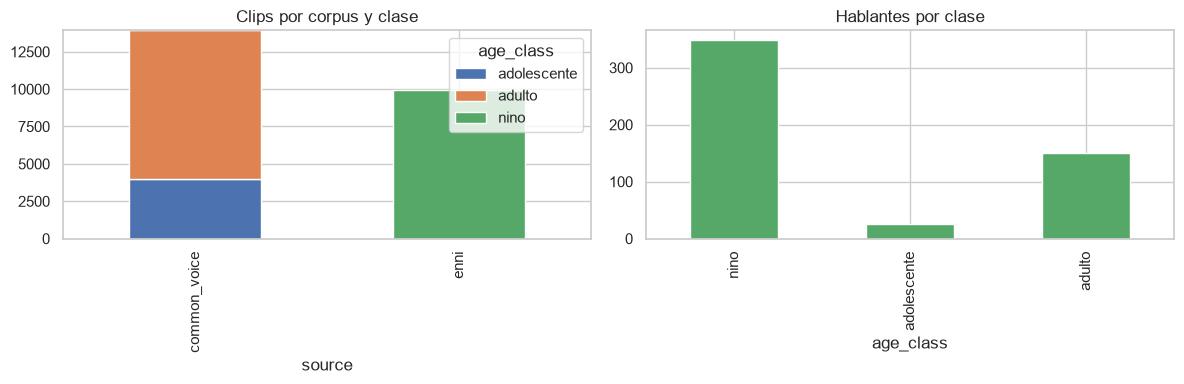
\includegraphics[width=0.9\linewidth]{figuras/clips_corpus_hablantes_clase.png}
\caption{Fragmentos por corpus y clase, y número de hablantes (o pseudo-hablantes) por clase en el conjunto unido.}
\label{fig:corpus_clase}
\end{figure}

\begin{figure}[H]
\centering
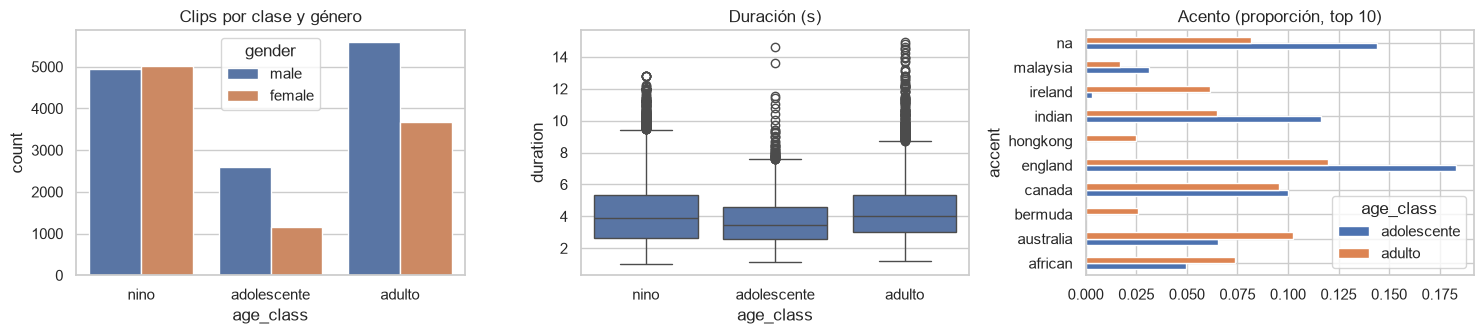
\includegraphics[width=\linewidth]{figuras/dataset_clase_duracion_acento.png}
\caption{Conjunto unido: fragmentos por clase y género, duración por clase y proporción de los diez acentos más frecuentes en adolescentes y adultos.}
\label{fig:dataset}
\end{figure}

\textbf{Partición por hablante.} Ningún hablante aparece en dos particiones; si apareciera, el modelo memorizaría voces y las métricas saldrían infladas. Se reparten hablantes completos en proporción aproximada 70/15/15 (figura~\ref{fig:particiones}).

\begin{figure}[H]
\centering
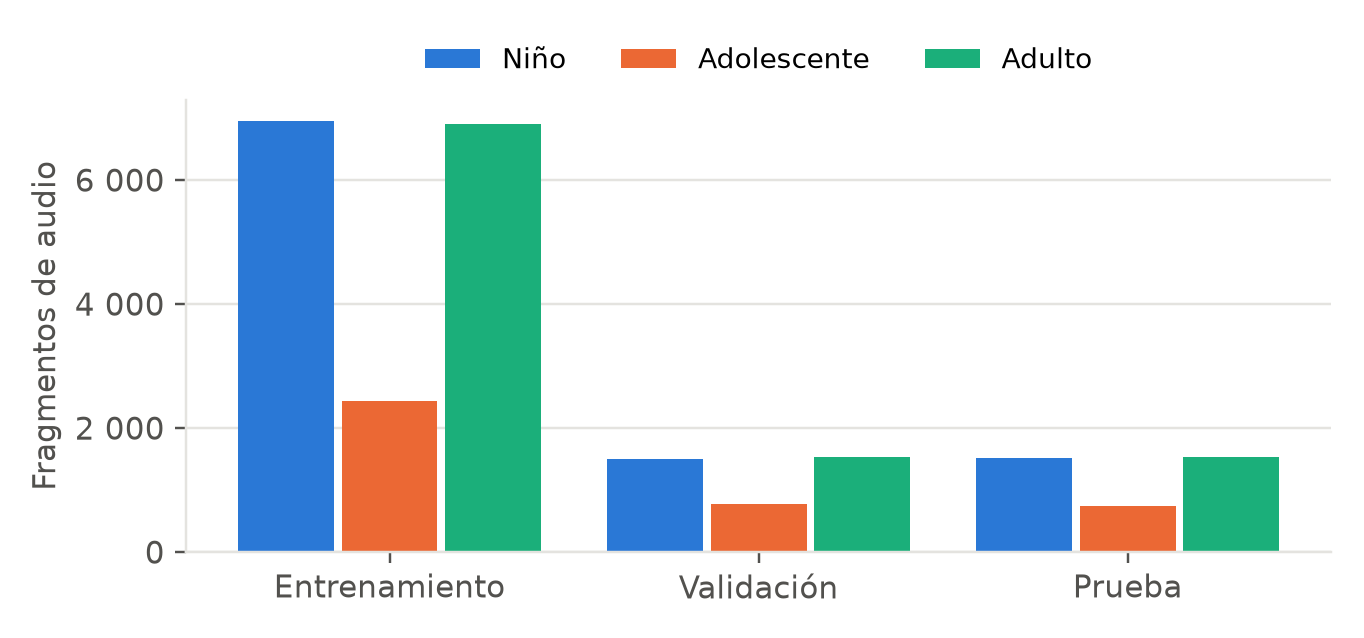
\includegraphics[width=0.78\linewidth]{figuras/particiones.png}
\caption{Fragmentos por clase en cada partición. En prueba hay 53 niños, 4 grupos de adolescentes y 24 grupos de adultos.}
\label{fig:particiones}
\end{figure}

\subsection{Flujo del sistema}

\begin{figure}[H]
\centering
\begin{tikzpicture}[
  caja/.style={draw=tinta, fill=fondo, rounded corners=3pt, align=center, font=\small, minimum height=1.05cm, text width=2.7cm},
  flecha/.style={-{Stealth[length=2.2mm]}, thick, tinta}]
\node[caja] (a) {Audio de la\\conversación};
\node[caja, right=0.45cm of a] (b) {Detección de\\voz y diarización};
\node[caja, right=0.45cm of b] (c) {Edad por\\hablante};
\node[caja, right=0.45cm of c] (d) {Puntaje y\\nivel de riesgo};
\node[caja, below=0.7cm of d, fill=white] (e) {Revisión\\humana};
\draw[flecha] (a) -- (b); \draw[flecha] (b) -- (c); \draw[flecha] (c) -- (d); \draw[flecha] (d) -- (e);
\node[font=\scriptsize, text=tinta, below=0.08cm of b, text width=2.6cm, align=center] {¿quién habla\\y cuándo?};
\node[font=\scriptsize, text=tinta, below=0.08cm of c, text width=2.6cm, align=center] {P(niño), P(adol.),\\P(adulto)};
\end{tikzpicture}
\caption{Flujo de punta a punta. El contenido de lo que se dice nunca se analiza.}
\end{figure}

\begin{enumerate}
  \item \textbf{Carga y normalización:} audio mono a 16\,kHz con el volumen igualado, para que el modelo no aprenda que una fuente está grabada más fuerte que otra.
  \item \textbf{Detección de actividad de voz} por energía, para quitar los silencios.
  \item \textbf{Diarización:} el audio se corta en ventanas de 1,5\,s, a cada ventana se le calcula un vector de hablante (ECAPA-TDNN) y las ventanas se agrupan por similitud. Cada grupo es un hablante. Si se conoce el número de participantes, puede indicarse.
  \item \textbf{Estimación de edad:} el audio de cada hablante se divide en trozos de hasta 6\,s, el modelo estima las probabilidades de cada trozo y se promedian según su duración.
  \item \textbf{Riesgo:} se combinan las probabilidades de todos los pares de hablantes (sección~\ref{sec:riesgo}).
\end{enumerate}

\subsection{Preprocesamiento y aumentación de datos}

Antes de extraer características, cada fragmento se recorta a sus primeros 8\,s, se normaliza y se le quitan los silencios; los que quedan con menos de 1\,s de voz se descartan. Para el entrenamiento, cada fragmento recibe además una \textbf{copia degradada} al azar: canal telefónico (filtro de 300--3400\,Hz), ruido de fondo con relación señal-ruido de 10 a 30\,dB o saturación de micrófono barato. La aumentación se aplica por igual a todas las clases, para que ``audio ruidoso'' no se vuelva pista de clase. \textbf{No se usa cambio de tono}, porque alteraría justo la señal de la edad.

\subsection{Extracción de características}

Cada fragmento se convierte en un vector numérico de longitud fija con tres extractores distintos, de lo más interpretable a lo más potente:

\begin{table}[H]
\centering
\caption{Extractores de características.}
\small
\begin{tabularx}{\linewidth}{@{}>{\raggedright\arraybackslash}p{2.9cm}cLc@{}}
\toprule
\textbf{Extractor} & \textbf{Dimensiones} & \textbf{Qué representa} & \textbf{Tiempo (ms)} \\
\midrule
Acústico clásico & 118 & Tono (frecuencia fundamental), formantes F1--F3, MFCC y rasgos espectrales & 16 \\
ECAPA-TDNN~\cite{ecapa2020} & 192 & ``Huella vocal'' de una red entrenada para reconocer hablantes (SpeechBrain~\cite{speechbrain2021}, VoxCeleb) & 29 \\
WavLM-base-plus~\cite{wavlm2022} & 1\,536 & Media y desviación estándar de las capas 3--8 del modelo autosupervisado & 89 \\
\bottomrule
\end{tabularx}
\end{table}

La figura~\ref{fig:f0} confirma en nuestros datos lo que predice el marco teórico: los niños tienen un tono claramente más alto (mediana de 242\,Hz), mientras que los adolescentes y los adultos se superponen casi por completo (147 y 154\,Hz).

\begin{figure}[H]
\centering
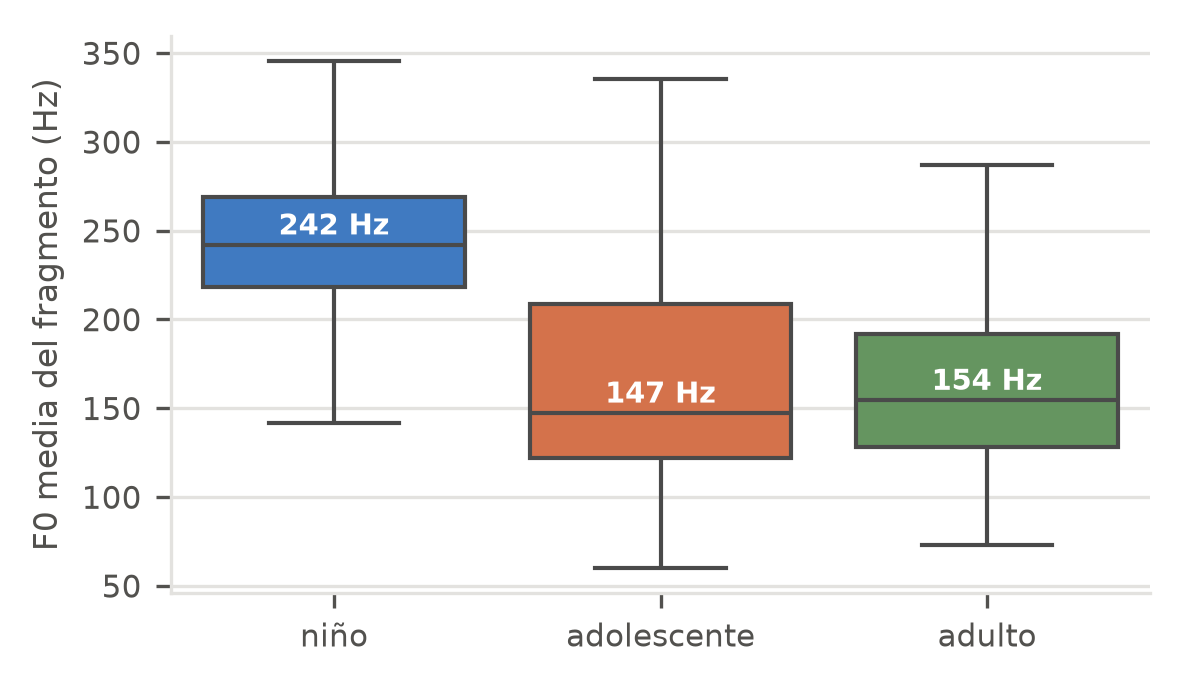
\includegraphics[width=0.78\linewidth]{figuras/f0_por_clase.png}
\caption{Tono fundamental medio por clase de edad, en todo el conjunto de datos.}
\label{fig:f0}
\end{figure}

\subsection{Modelos comparados}

Se entrenaron seis modelos, cada uno formado por una representación y un clasificador. Los tres principales (A, B, C) cubren de lo más interpretable a lo más potente; los otros tres son variantes que permiten separar qué aporta la representación y qué aporta el clasificador.

\begin{table}[H]
\centering
\caption{Modelos comparados y justificación.}
\small
\begin{tabularx}{\linewidth}{@{}p{0.5cm}>{\raggedright\arraybackslash}p{2.7cm}>{\raggedright\arraybackslash}p{2.7cm}L@{}}
\toprule
& \textbf{Representación} & \textbf{Clasificador} & \textbf{Por qué} \\
\midrule
A & Acústica clásica & Potenciación del gradiente~\cite{sklearn2011} & La fisiología explica la edad. Los árboles capturan umbrales no lineales (``tono alto y formantes altos $\Rightarrow$ niño''), son interpretables y corren en cualquier computadora. \\
B & ECAPA-TDNN & SVM con núcleo RBF & ECAPA es el estado del arte en reconocimiento de hablante; su vector resume tamaño del tracto vocal, timbre y tono. Es compacto, y la SVM generaliza bien con pocos datos de menores gracias al margen máximo. Además, el mismo vector sirve para la diarización. \\
C & WavLM & Regresión logística & Un clasificador lineal sobre el modelo congelado evita el sobreajuste con pocos datos y permite entrenar en una computadora personal. \\
A2 & Acústica clásica & Bosque aleatorio & Línea base liviana sin redes neuronales; ¿aporta la potenciación frente a árboles independientes? \\
A3 & Acústica clásica & Regresión logística & Piso de referencia: ¿basta un modelo lineal sobre rasgos fisiológicos? \\
B2 & ECAPA-TDNN & Bosque aleatorio & Misma representación que B con otro clasificador. \\
\bottomrule
\end{tabularx}
\end{table}

\subsection{Protocolo de entrenamiento}

Todos los modelos siguen el mismo protocolo, para que la comparación sea justa:
\begin{itemize}
  \item \textbf{Pesos de clase balanceados}, porque hay menos adolescentes.
  \item \textbf{Hiperparámetros} elegidos con una búsqueda en cuadrícula sobre el conjunto de validación, usando F1-macro.
  \item \textbf{Calibración sigmoide} sobre validación.
  \item \textbf{Evaluación una sola vez} en el conjunto de prueba, con hablantes que el modelo nunca vio.
  \item \textbf{Selección} del ganador por F1-macro en prueba; en caso de empate, gana el de mayor sensibilidad para niños.
\end{itemize}

\subsection{Puntaje de riesgo}
\label{sec:riesgo}

Para cada par de hablantes distintos $i$ (posible menor) y $j$ (posible adulto):
\begin{equation}
r(i,j) = P_i(\text{niño})\,P_j(\text{adulto}) \cdot 0{,}90 \;+\; P_i(\text{adolescente})\,P_j(\text{adulto}) \cdot 0{,}60
\end{equation}
El riesgo del audio es el máximo sobre todos los pares, porque basta una pareja menor--adulto para alertar, con un piso de 0,05 para no afirmar nunca ``riesgo cero''. Los niveles son \textbf{bajo} ($<0{,}30$), \textbf{medio} ($0{,}30$--$0{,}60$) y \textbf{alto} ($\geq 0{,}60$). Los pesos (0,90 y 0,60) reflejan que la pareja niño--adulto es la de mayor preocupación y que la etiqueta de adolescente es menos fiable. Por ejemplo, si un hablante es niño con 95\,\% de probabilidad y otro adulto con 90\,\%, el riesgo es $0{,}95 \times 0{,}90 \times 0{,}90 \approx 0{,}77$. Si el modelo duda, el riesgo baja en proporción.

\subsection{Implementación y despliegue}

El sistema está escrito en Python como un paquete compartido por el cuaderno de entrenamiento y el servicio. El modelo ganador se sirve mediante una API web (FastAPI) en un contenedor Docker que funciona sin conexión a internet y solo con CPU. La ruta \texttt{/analyze} recibe un archivo de audio de hasta 10 minutos y devuelve el puntaje de riesgo (0 a 1), su nivel, el número de hablantes detectados y, para cada uno, su duración, sus intervalos de habla y sus probabilidades de edad. Todas las respuestas incluyen un \textbf{aviso obligatorio} de que el resultado es una alerta y no un veredicto. El audio se procesa en un archivo temporal que se borra al terminar: el servicio no conserva grabaciones ni transcripciones.

%=====================================================================
\section{Resultados}
%=====================================================================

\subsection{Comparativa de modelos}

El modelo B (ECAPA-TDNN + SVM, con $C=0{,}3$) obtuvo el mejor F1-macro y la mejor sensibilidad para adolescentes, y es el que se usa en el sistema (tabla~\ref{tab:resultados} y figura~\ref{fig:modelos}). La evaluación usa 3\,724 fragmentos de hablantes nunca vistos.

\begin{table}[H]
\centering
\caption{Resultados en el conjunto de prueba (por fragmento). En negritas, el mejor valor.}
\label{tab:resultados}
\footnotesize
\setlength{\tabcolsep}{4pt}
\begin{tabular}{@{}lcccccc@{}}
\toprule
\textbf{Modelo} & \textbf{F1-macro} & \textbf{Exact. bal.} & \textbf{Sens. niño} & \textbf{Sens. adol.} & \textbf{Sens. adulto} & \textbf{AUC} \\
\midrule
B ECAPA + SVM          & \textbf{0,817} & \textbf{0,814} & 0,987 & \textbf{0,604} & 0,852 & \textbf{0,943} \\
C WavLM + reg. log.    & 0,786 & 0,778 & \textbf{1,000} & 0,427 & 0,906 & 0,940 \\
B2 ECAPA + bosque      & 0,776 & 0,768 & 0,965 & 0,430 & 0,910 & 0,941 \\
A2 Acústico + bosque   & 0,730 & 0,728 & 0,994 & 0,308 & 0,884 & 0,900 \\
A Acústico + pot. grad.& 0,708 & 0,710 & 0,997 & 0,261 & 0,872 & 0,870 \\
A3 Acústico + reg. log.& 0,598 & 0,658 & 0,999 & 0,010 & \textbf{0,965} & 0,872 \\
\bottomrule
\end{tabular}

\vspace{2pt}
{\footnotesize Sens. = sensibilidad. AUC = área bajo la curva para separar menores de adultos.}
\end{table}

\begin{figure}[H]
\centering
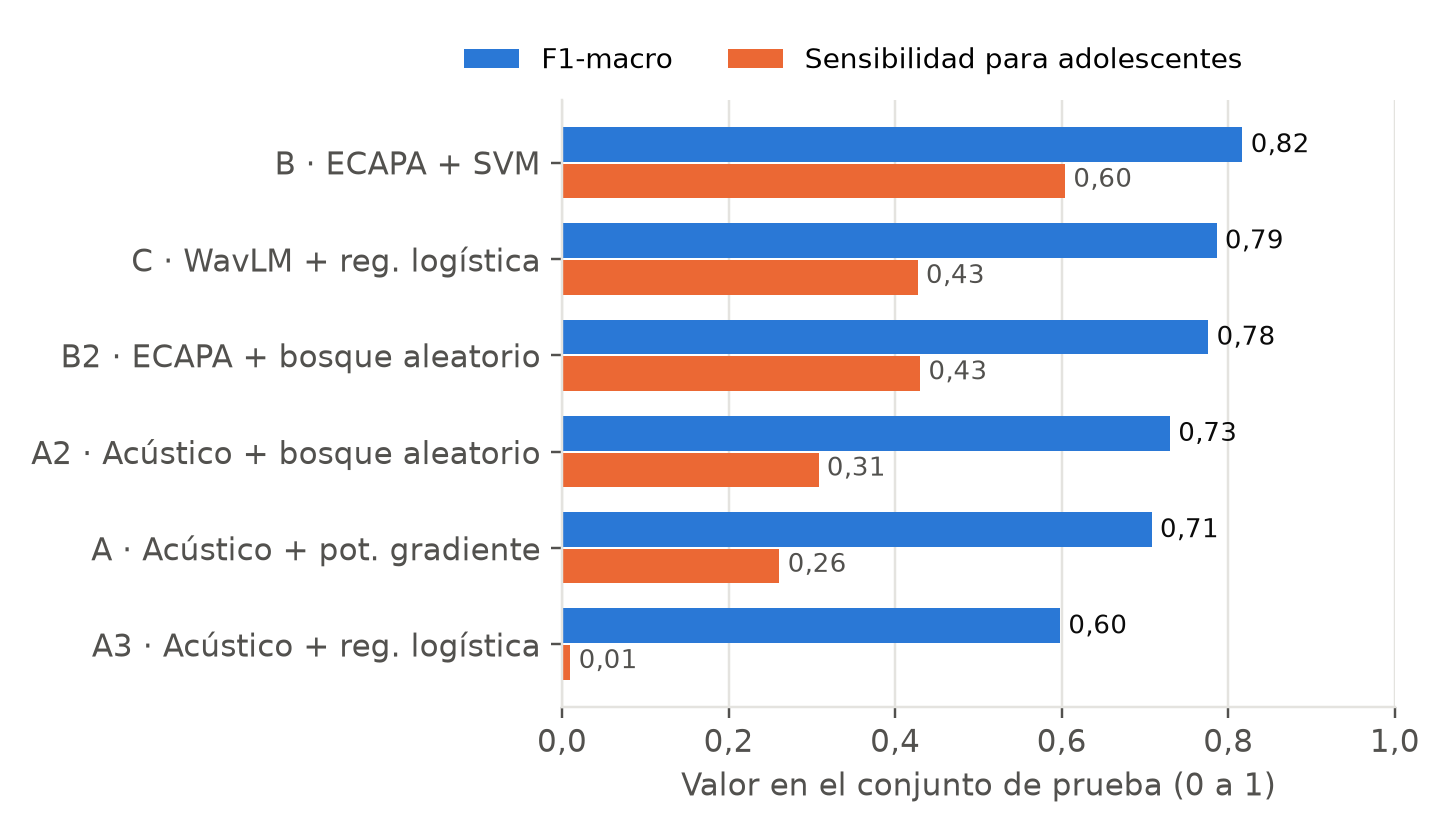
\includegraphics[width=0.82\linewidth]{figuras/comparativa_modelos.png}
\caption{F1-macro y sensibilidad para adolescentes de cada modelo.}
\label{fig:modelos}
\end{figure}

\textbf{Lecturas principales.}
\begin{itemize}
  \item \textbf{La representación pesa más que el clasificador.} Con rasgos acústicos el mejor modelo llega a 0,730; con ECAPA, incluso un bosque aleatorio sube a 0,776.
  \item \textbf{Con ECAPA, la SVM supera al bosque aleatorio} (0,817 frente a 0,776), y la diferencia está en los adolescentes (0,604 frente a 0,430).
  \item \textbf{Un modelo lineal sobre rasgos acústicos casi no detecta adolescentes} (0,010): como muestra la figura~\ref{fig:f0}, su tono es casi igual al de los adultos, y la frontera entre ambas clases no es lineal.
  \item \textbf{El error típico del modelo B es confundir adolescentes con adultos} (39\,\% de los fragmentos adolescentes se clasifican como adultos); casi nunca confunde a un niño con un adulto (figura~\ref{fig:confusion}).
  \item \textbf{La sensibilidad para niños (0,97--1,00) debe leerse con cautela}: todos los niños provienen de habla sintetizada (sección~\ref{sec:sesgo}).
\end{itemize}

\begin{figure}[H]
\centering
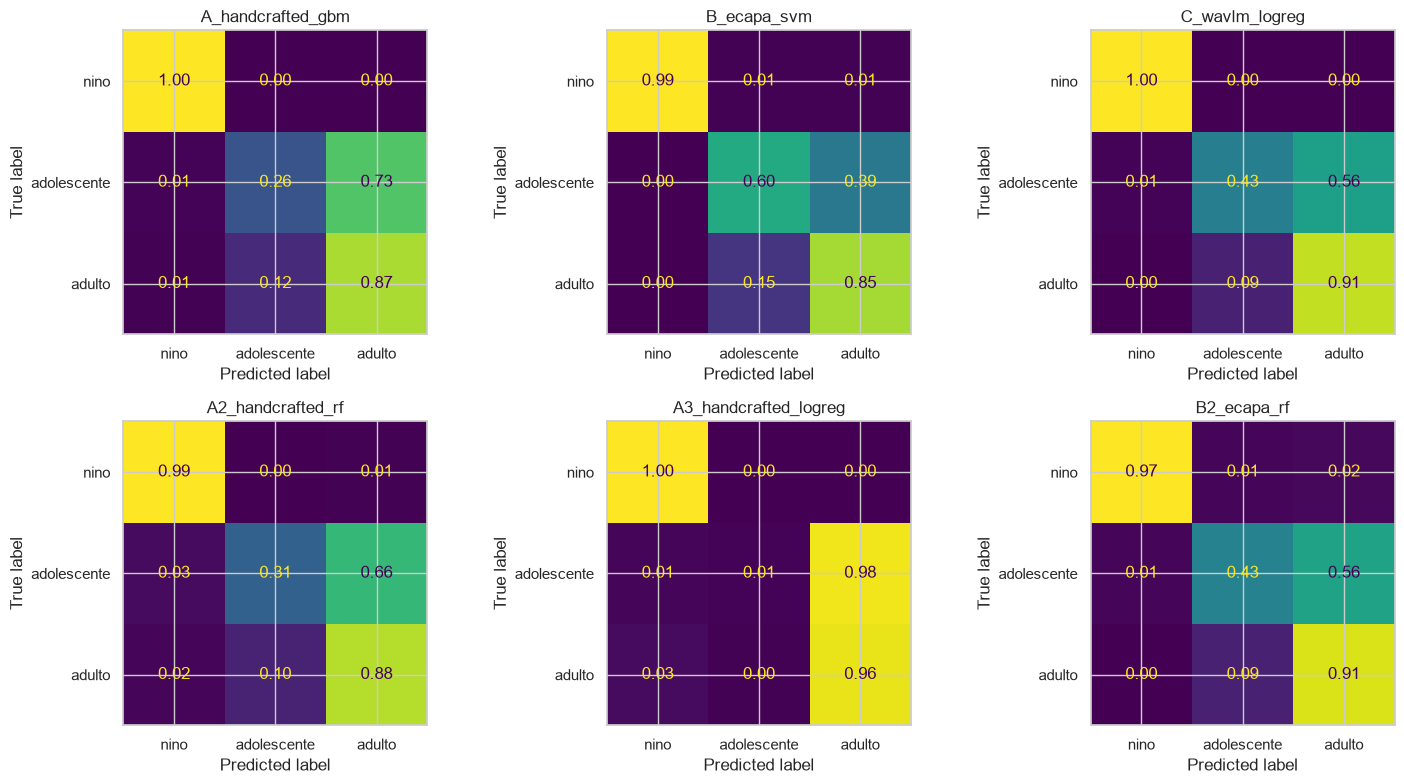
\includegraphics[width=\linewidth]{figuras/matrices_confusion.png}
\caption{Matrices de confusión normalizadas por clase real (filas) en el conjunto de prueba, para los seis modelos. La diagonal es la sensibilidad de cada clase.}
\label{fig:confusion}
\end{figure}

\textbf{Resultados por hablante.} Al promediar las predicciones de todos los fragmentos de cada hablante, el modelo B alcanza un F1-macro de 0,837, una exactitud balanceada de 0,819 y un AUC de 0,998; detecta al 100\,\% de los niños y al 95,8\,\% de los adultos. La sensibilidad para adolescentes es de 0,50, pero se calcula sobre solo 4 grupos de adolescentes en prueba, por lo que es muy imprecisa.

\subsection{Eficiencia}

El costo de inferencia lo pone casi por completo el extractor, no el clasificador:

\begin{table}[H]
\centering
\caption{Tiempo de inferencia por fragmento en CPU y tamaño.}
\small
\begin{tabular}{@{}lcccc@{}}
\toprule
\textbf{Modelo} & \textbf{F1-macro} & \textbf{ms/fragmento} & \textbf{Clasificador (MB)} & \textbf{Red (MB)} \\
\midrule
B ECAPA + SVM         & 0,817 & 29 & 15,9 & 83 \\
C WavLM + reg. log.   & 0,786 & 89 & 0,1 & 378 \\
A2 Acústico + bosque  & 0,730 & 16 & 35,9 & 0 \\
\bottomrule
\end{tabular}
\end{table}

El modelo A2 es la mejor opción sin redes neuronales y tarda la mitad que B. Pero el sistema necesita ECAPA de todos modos para la diarización, así que cambiar a A2 casi no ahorraría recursos y costaría 0,09 de F1-macro y la mitad de la sensibilidad para adolescentes. Ya desplegado, tras la carga inicial del modelo, analizar una conversación de 10\,s tomó menos de 0,2\,s.

\subsection{Auditoría de sesgo por canal}
\label{sec:sesgo}

El mayor riesgo metodológico es que \textbf{clase y fuente coinciden}: todos los niños vienen de habla sintetizada y limpia, y todos los demás de grabaciones caseras. El modelo podría aprender ``qué tipo de audio es'' en lugar de ``qué edad tiene''. Se hicieron tres comprobaciones:

\begin{itemize}
  \item \textbf{Diferencias de canal:} los audios infantiles eran unos 13\,dB más bajos y con distinto espectro (figura~\ref{fig:canal}). La diferencia de volumen se elimina con la normalización; la de espectro, no.
  \item \textbf{Predictibilidad de la fuente:} un clasificador simple adivina la fuente en el 98,8\,\% de los casos con los vectores ECAPA (57,9\,\% por azar). Con estos datos es inevitable, porque predecir la fuente equivale a predecir ``niño''.
  \item \textbf{Robustez al canal:} se degradó el audio de prueba con ruido y canal telefónico. Si el modelo usara ``audio limpio = niño'', su sensibilidad para niños se desplomaría.
\end{itemize}

\begin{figure}[H]
\centering
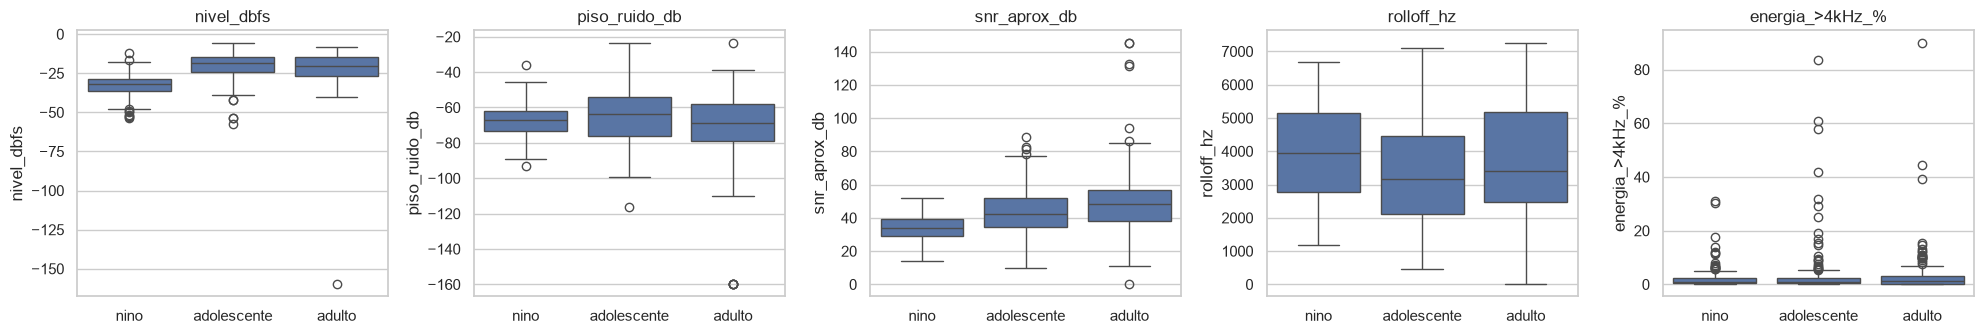
\includegraphics[width=\linewidth]{figuras/dataset_canal_por_clase.png}
\caption{Rasgos de canal por clase, en una muestra de 150 fragmentos por clase antes de normalizar: nivel (dBFS), piso de ruido, relación señal-ruido aproximada, frecuencia de corte espectral (\emph{rolloff}) y porcentaje de energía por encima de 4\,kHz.}
\label{fig:canal}
\end{figure}

\begin{table}[H]
\centering
\caption{Modelo B con audio de prueba original y degradado.}
\small
\begin{tabular}{@{}lccccc@{}}
\toprule
\textbf{Audio} & \textbf{F1-macro} & \textbf{Sens. niño} & \textbf{Sens. adol.} & \textbf{Sens. adulto} & \textbf{AUC} \\
\midrule
Original  & 0,817 & 0,987 & 0,604 & 0,852 & 0,943 \\
Degradado & 0,813 & 0,979 & 0,567 & 0,876 & 0,944 \\
\bottomrule
\end{tabular}
\end{table}

\textbf{Conclusión:} el modelo no depende de que el audio sea limpio, pero todavía podría apoyarse en que la voz infantil es sintetizada. Para descartarlo hace falta un corpus con niños y adultos reales grabados en las mismas condiciones.

\subsection{Conversaciones simuladas}

Para probar el sistema completo se armaron conversaciones alternando turnos de hablantes de prueba, 20 por escenario:

\begin{table}[H]
\centering
\caption{Resultados del flujo completo con conversaciones simuladas.}
\small
\begin{tabular}{@{}lccc@{}}
\toprule
\textbf{Escenario} & \textbf{Riesgo medio} & \textbf{Alertas altas} & \textbf{Hablantes detectados (reales)} \\
\midrule
Niño + adulto        & 0,585 & 80\,\% & 3,3 (2) \\
Adolescente + adulto & 0,231 & 0\,\%  & 2,1 (2) \\
Adulto + adulto      & 0,183 & 0\,\%  & 2,4 (2) \\
Niño + niño          & 0,084 & 0\,\%  & 3,9 (2) \\
Adulto solo          & 0,068 & 0\,\%  & 1,2 (1) \\
\bottomrule
\end{tabular}
\end{table}

\begin{figure}[H]
\centering
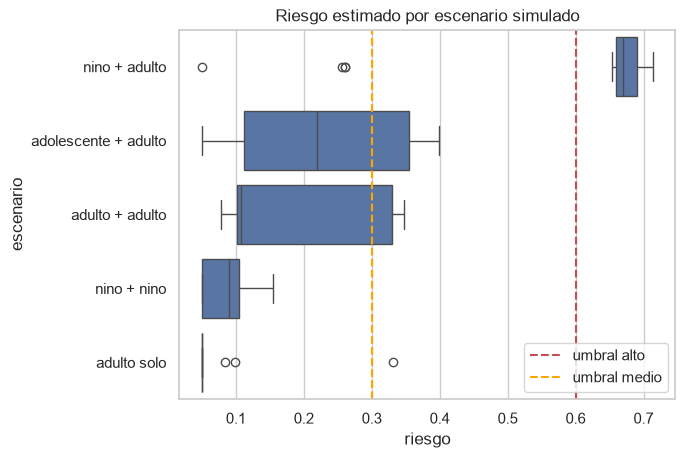
\includegraphics[width=0.75\linewidth]{figuras/riesgo_escenarios_simulados.png}
\caption{Distribución del riesgo estimado en las conversaciones simuladas, por escenario. Las líneas punteadas marcan los umbrales de riesgo medio (0,30) y alto (0,60).}
\label{fig:simuladas}
\end{figure}

\begin{itemize}
  \item \textbf{Las conversaciones entre niño y adulto generan alerta alta en el 80\,\% de los casos} (figura~\ref{fig:simuladas}). Ningún otro escenario llega a alerta alta, aunque algunas conversaciones adolescente + adulto y adulto + adulto alcanzan riesgo medio.
  \item \textbf{La diarización cuenta hablantes de más cuando hay niños}, porque cada fragmento sintetizado suena como una voz distinta. Eso reparte al niño entre varios hablantes falsos y baja el riesgo medio. Indicar el número de participantes corrige el problema: con dos hablantes indicados, una conversación de prueba niño--adulto obtuvo 71\,\% (alto), con el niño identificado al 87\,\% y el adulto al 84\,\%.
  \item \textbf{``Adolescente + adulto'' casi nunca alerta}, consecuencia directa de la baja sensibilidad para adolescentes.
\end{itemize}

\subsection{Pruebas del sistema}

\begin{table}[H]
\centering
\caption{Resumen de pruebas.}
\small
\begin{tabularx}{\linewidth}{@{}>{\raggedright\arraybackslash}p{4cm}L>{\raggedright\arraybackslash}p{2.6cm}@{}}
\toprule
\textbf{Prueba} & \textbf{Qué verifica} & \textbf{Resultado} \\
\midrule
Pruebas unitarias (15 casos) & Fronteras de edad; riesgo de 90\,\% para niño + adulto y de 60\,\% para adolescente + adulto; piso sin pareja menor--adulto; escalado con la incertidumbre & 15/15 correctas \\
Ausencia de fuga de hablantes & Ningún hablante en dos particiones & Verificada \\
Calidad de datos & Eliminación de fragmentos mudos y verificación de etiquetas & 13 mudos eliminados \\
Entrenamiento completo & Todo el proceso de principio a fin & Sin errores \\
API local y en contenedor & Respuestas idénticas en ambos entornos, aviso presente & Correcta \\
\bottomrule
\end{tabularx}
\end{table}

%=====================================================================
\section{Trabajo a futuro}
%=====================================================================

Los resultados muestran que es posible estimar, solo con la voz, si en una conversación hablan un menor y un adulto, pero el sistema todavía no está listo para un uso real. La tabla~\ref{tab:futuro} resume sus limitaciones y las mejoras propuestas.

\begin{table}[H]
\centering
\caption{Limitaciones conocidas y mejoras propuestas.}
\label{tab:futuro}
\small
\begin{tabularx}{\linewidth}{@{}>{\raggedright\arraybackslash}p{4cm}L>{\raggedright\arraybackslash}p{4.3cm}@{}}
\toprule
\textbf{Limitación} & \textbf{Efecto} & \textbf{Mejora} \\
\midrule
Todos los niños provienen de habla sintetizada & El rendimiento con niños puede estar inflado & Corpus con niños y adultos reales en el mismo canal (speechocean762, MyST, CSLU Kids) \\
Pocos adolescentes (25 grupos) & Sensibilidad de 0,60; casi no hay alertas adolescente--adulto & Más datos de adolescentes con edad exacta \\
``Teens'' en Common Voice incluye 18 y 19 años & Etiquetas ruidosas & Corpus con edad exacta \\
Solo inglés & Rendimiento desconocido en español & Añadir voces en español \\
Diarización ligera & Cuenta hablantes de más con voces infantiles & Diarización neuronal (pyannote, NeMo) \\
Evaluación con conversaciones simuladas & Resultados optimistas & Validación con conversaciones reales anotadas, con consentimiento \\
\bottomrule
\end{tabularx}
\end{table}

Además:
\begin{itemize}
  \item \textbf{Ajuste fino de WavLM.} Con más datos de menores, el siguiente paso natural es ajustar finamente WavLM en lugar de usarlo congelado.
  \item \textbf{Calibración de umbrales.} Los pesos y umbrales del riesgo se fijaron por diseño; deben recalibrarse con conversaciones reales y documentarse cada cambio.
  \item \textbf{Condiciones para un despliegue real.} Requeriría base legal, aviso o consentimiento adecuado, una evaluación de impacto en protección de datos y un equipo de revisión humana especializada. Ninguna acción con consecuencias debe acoplarse automáticamente al puntaje, y debe asumirse que la mayoría de las alertas corresponderán a conversaciones legítimas.
\end{itemize}

%=====================================================================
\section{Declaración de uso de IA}
%=====================================================================

\aviso{\textbf{Pendiente.} Esta sección se completará más adelante.}

%=====================================================================
\begin{thebibliography}{99}
\small

\bibitem{whittle2013} H.~Whittle, C.~Hamilton-Giachritsis, A.~Beech y G.~Collings. ``A review of online grooming: Characteristics and concerns''. \emph{Aggression and Violent Behavior}, 18(1):62--70, 2013.

\bibitem{ncmec2025} National Center for Missing \& Exploited Children. ``NCMEC Releases New Data: 2024 in Numbers'', 2025. \url{https://www.missingkids.org/blog/2025/ncmec-releases-new-data-2024-in-numbers}

\bibitem{thorn2025} Thorn. ``What the 2024 NCMEC CyberTipline Report Says About Child Safety'', 2025. \url{https://www.thorn.org/blog/what-the-2024-ncmec-cybertipline-report-says-about-child-safety/}

\bibitem{nspcc2025} NSPCC. ``Data shows how criminals are using private messaging platforms to manipulate and groom children'', noviembre de 2025. \url{https://www.nspcc.org.uk/about-us/news-opinion/2025/data-shows-how-criminals-are-using-private-messaging-platforms-to-manipulate-and-groom-children/}

\bibitem{weprotect2023} WeProtect Global Alliance. \emph{Global Threat Assessment 2023}. \url{https://www.weprotect.org/global-threat-assessment-23/}

\bibitem{inegi2025} INEGI. \emph{Módulo sobre Ciberacoso (MOCIBA) 2024}, comunicado de prensa 76/25, 17 de julio de 2025. \url{https://www.inegi.org.mx/programas/mociba/2024/}

\bibitem{edpb2022} EDPB y EDPS. \emph{Joint Opinion 4/2022 on the Proposal for a Regulation laying down rules to prevent and combat child sexual abuse}, 28 de julio de 2022. \url{https://edps.europa.eu/data-protection/our-work/publications/edps-edpb-joint-opinions/2022-07-28-joint-opinion-42022-regulation-european-parliament-and-council-rules-prevent-and-combat-child-sexual-abuse_en}

\bibitem{pan2012} G.~Inches y F.~Crestani. ``Overview of the International Sexual Predator Identification Competition at PAN-2012''. \emph{CLEF 2012 Evaluation Labs and Workshop}, 2012.

\bibitem{villatoro2012} E.~Villatoro-Tello, A.~Juárez-González, H.~J.~Escalante, M.~Montes-y-Gómez y L.~Villaseñor-Pineda. ``A two-step approach for effective detection of misbehaving users in chats''. \emph{CLEF 2012 Evaluation Labs and Workshop}, 2012.

\bibitem{ebrahimi2016} M.~Ebrahimi, C.~Y.~Suen y O.~Ormandjieva. ``Detecting predatory conversations in social media by deep convolutional neural networks''. \emph{Digital Investigation}, 18:33--49, 2016.

\bibitem{metze2007} F.~Metze, J.~Ajmera, R.~Englert, U.~Bub, F.~Burkhardt, J.~Stegmann, C.~Müller, R.~Huber, B.~Andrassy, J.~G.~Bauer y B.~Littel. ``Comparison of four approaches to age and gender recognition for telephone applications''. \emph{IEEE ICASSP}, 2007.

\bibitem{schuller2010} B.~Schuller, S.~Steidl, A.~Batliner, F.~Burkhardt, L.~Devillers, C.~Müller y S.~Narayanan. ``The INTERSPEECH 2010 Paralinguistic Challenge''. \emph{Interspeech}, 2010.

\bibitem{bahari2014} M.~H.~Bahari, M.~McLaren, H.~Van~hamme y D.~A.~van~Leeuwen. ``Speaker age estimation using i-vectors''. \emph{Engineering Applications of Artificial Intelligence}, 34:99--108, 2014.

\bibitem{ghahremani2018} P.~Ghahremani, P.~S.~Nidadavolu, N.~Chen, J.~Villalba, D.~Povey, S.~Khudanpur y N.~Dehak. ``End-to-end deep neural network age estimation''. \emph{Interspeech}, 2018.

\bibitem{xvector2018} D.~Snyder, D.~Garcia-Romero, G.~Sell, D.~Povey y S.~Khudanpur. ``X-vectors: Robust DNN embeddings for speaker recognition''. \emph{IEEE ICASSP}, 2018.

\bibitem{burkhardt2023} F.~Burkhardt, J.~Wagner, H.~Wierstorf, F.~Eyben y B.~Schuller. ``Speech-based age and gender prediction with transformers''. \emph{ITG Conference on Speech Communication}, 2023.

\bibitem{park2022} T.~J.~Park, N.~Kanda, D.~Dimitriadis, K.~J.~Han, S.~Watanabe y S.~Narayanan. ``A review of speaker diarization: Recent advances with deep learning''. \emph{Computer Speech \& Language}, 72:101317, 2022.

\bibitem{pyannote2020} H.~Bredin et~al. ``pyannote.audio: neural building blocks for speaker diarization''. \emph{IEEE ICASSP}, 2020.

\bibitem{fant1960} G.~Fant. \emph{Acoustic Theory of Speech Production}. Mouton, La Haya, 1960.

\bibitem{lee1999} S.~Lee, A.~Potamianos y S.~Narayanan. ``Acoustics of children's speech: Developmental changes of temporal and spectral parameters''. \emph{Journal of the Acoustical Society of America}, 105(3):1455--1468, 1999.

\bibitem{davis1980} S.~Davis y P.~Mermelstein. ``Comparison of parametric representations for monosyllabic word recognition in continuously spoken sentences''. \emph{IEEE Transactions on Acoustics, Speech, and Signal Processing}, 28(4):357--366, 1980.

\bibitem{enni2005} P.~Schneider, R.~V.~Dubé y D.~Hayward. \emph{The Edmonton Narrative Norms Instrument}. University of Alberta, 2005.

\bibitem{enniHF} jsun39. \emph{enni-child-speech-synthesis} (conjunto de datos). Hugging Face. \url{https://huggingface.co/datasets/jsun39/enni-child-speech-synthesis}

\bibitem{commonvoice2020} R.~Ardila et~al. ``Common Voice: A Massively-Multilingual Speech Corpus''. \emph{Proceedings of LREC}, 2020.

\bibitem{ecapa2020} B.~Desplanques, J.~Thienpondt y K.~Demuynck. ``ECAPA-TDNN: Emphasized Channel Attention, Propagation and Aggregation in TDNN Based Speaker Verification''. \emph{Interspeech}, 2020.

\bibitem{speechbrain2021} M.~Ravanelli et~al. ``SpeechBrain: A General-Purpose Speech Toolkit''. arXiv:2106.04624, 2021.

\bibitem{wavlm2022} S.~Chen et~al. ``WavLM: Large-Scale Self-Supervised Pre-Training for Full Stack Speech Processing''. \emph{IEEE Journal of Selected Topics in Signal Processing}, 16(6), 2022.

\bibitem{superb2021} S.~Yang et~al. ``SUPERB: Speech processing Universal PERformance Benchmark''. \emph{Interspeech}, 2021.

\bibitem{svm1995} C.~Cortes y V.~Vapnik. ``Support-vector networks''. \emph{Machine Learning}, 20:273--297, 1995.

\bibitem{rf2001} L.~Breiman. ``Random Forests''. \emph{Machine Learning}, 45:5--32, 2001.

\bibitem{friedman2001} J.~H.~Friedman. ``Greedy function approximation: A gradient boosting machine''. \emph{Annals of Statistics}, 29(5):1189--1232, 2001.

\bibitem{platt1999} J.~Platt. ``Probabilistic outputs for support vector machines and comparisons to regularized likelihood methods''. \emph{Advances in Large Margin Classifiers}, 1999.

\bibitem{sklearn2011} F.~Pedregosa et~al. ``Scikit-learn: Machine Learning in Python''. \emph{Journal of Machine Learning Research}, 12:2825--2830, 2011.

\end{thebibliography}

\end{document}
